\documentclass{article}

% Required packages (merged from hw5_template.tex and hw6_questions.tex)
\usepackage{amssymb}
\usepackage{amsmath}
\usepackage{graphicx}
\usepackage{geometry}
\usepackage{tikz}
\usepackage{array}
\usepackage{booktabs}
\usepackage{enumitem}
\usepackage{listings}
\usepackage{xcolor}
\usepackage{fancyhdr}
\usepackage{float}
\usepackage{subcaption}
\usepackage{comment}
\usepackage{algorithm}
\usepackage{algpseudocode}
\usepackage{caption}
\usepackage{siunitx}
\usepackage{hyperref}
\usetikzlibrary{arrows.meta, positioning} % Required for hw6 diagrams

% Set page geometry
\geometry{a4paper, margin=1in}

% Configure listings for Python
\lstset{
  language=Python,
  basicstyle=\ttfamily\footnotesize,
  numbers=left,
  numberstyle=\tiny\color{gray},
  frame=single,
  breaklines=true,
  breakatwhitespace=true,
  captionpos=b,
  tabsize=4,
  showspaces=false,
  showstringspaces=false,
  showtabs=false,
  commentstyle=\color{gray}\textit,
  keywordstyle=\color{blue}\bfseries,
  stringstyle=\color{red}
}

\begin{document}

\pagestyle{fancy}
\chead{DSC 257: Unsupervised Learning (Fall 2025)}
\lhead{Homework 9}
\rhead{Randall Rogers}

%------------------
% Solution for 1(a)
%------------------
\subsection*{Solution 1}
\noindent\rule{\textwidth}{0.4pt}\\
\subsubsection*{Solution 1 (a)}
The function $\phi(x)$ returns the index $j$ corresponding to the closest cluster center. Since there are $k$ cluster centers indexed from $1$ to $k$, the output is a single discrete integer.

\subsubsection*{\normalfont}{$\therefore$ Thus, the space is the discrete set of indices:}
$$ \phi(x) \in \{1, 2, \ldots, k\} $$

\noindent\rule{\textwidth}{0.4pt}\\
\newpage

%------------------
% Solution for 1(b)
%------------------
\subsection*{Solution 1}
\noindent\rule{\textwidth}{0.4pt}\\
\subsubsection*{Solution 1 (b)}
Since distances in a metric space are non-negative real numbers, $\phi(x)$ is a vector in a $k$-dimensional Euclidean space (specifically the non-negative orthant).

\begin{center}
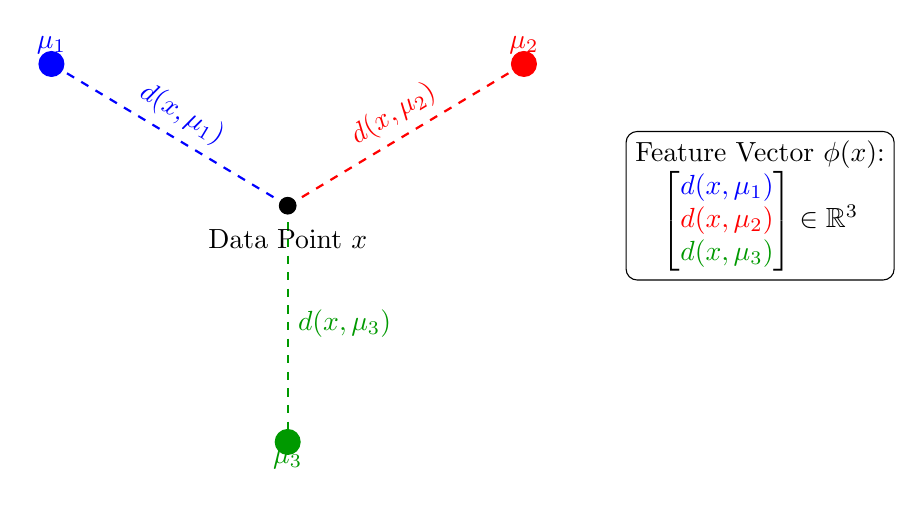
\begin{tikzpicture}[scale=1.5]
    % Define coordinates
    \coordinate (X) at (2, 2);
    \coordinate (Mu1) at (0, 3.2);
    \coordinate (Mu2) at (4, 3.2);
    \coordinate (Mu3) at (2, 0);

    % Draw connections (Distances)
    \draw[dashed, blue, thick] (X) -- (Mu1) node[midway, above, sloped] {$d(x, \mu_1)$};
    \draw[dashed, red, thick] (X) -- (Mu2) node[midway, above, sloped] {$d(x, \mu_2)$};
    \draw[dashed, green!60!black, thick] (X) -- (Mu3) node[midway, right] {$d(x, \mu_3)$};

    % Draw Points
    \filldraw[black] (X) circle (2pt) node[below=5pt] {Data Point $x$};
    
    % Draw Cluster Centers
    \filldraw[blue] (Mu1) circle (3pt) node[above] {$\mu_1$};
    \filldraw[red] (Mu2) circle (3pt) node[above] {$\mu_2$};
    \filldraw[green!60!black] (Mu3) circle (3pt) node[below] {$\mu_3$};
    
    % Annotate the resulting vector
    \node[align=center, draw, rectangle, rounded corners] at (6, 2) {
        Feature Vector $\phi(x)$: \\
        $\begin{bmatrix} 
        \textcolor{blue}{d(x, \mu_1)} \\ 
        \textcolor{red}{d(x, \mu_2)} \\ 
        \textcolor{green!60!black}{d(x, \mu_3)} 
        \end{bmatrix} \in \mathbb{R}^3$
    };
\end{tikzpicture}
\end{center}

\subsubsection*{\normalfont}{$\therefore \phi(x) \in \mathbb{R}^k$}

\noindent\rule{\textwidth}{0.4pt}\\

\newpage

%------------------
% Solution for 2
%------------------
\subsection*{Solution 2}
\noindent\rule{\textwidth}{0.4pt}\\
\subsubsection*{Question 2}
\begin{flushleft}
    Each of the following matrices gives distances (not squared distances) between a set of three points. In each case, say whether the distances can be realized in Euclidean space. If they can, show how by specifying three vectors with exactly the given interpoint distances. If they can't, give a reason.

\[
\begin{bmatrix}
0 & 1 & 2 \\
1 & 0 & 1 \\
2 & 1 & 0
\end{bmatrix}, \quad
\begin{bmatrix}
0 & 1 & 3 \\
1 & 0 & 1 \\
3 & 1 & 0
\end{bmatrix}
\]
\end{flushleft}

% CHANGED: Removed duplicate \subsection*{Solution 2} here
\subsubsection*{Answer} 
\begin{enumerate}
    \item Case 1: Matrix $D_1$
    \begin{flushleft}
        From the matrix, the distances are:
        $$ d(x_1, x_2) = 1, \quad d(x_2, x_3) = 1, \quad d(x_1, x_3) = 2$$
        Now, check the triangle inequality for the longest edge: 
        % FIXED TYPO BELOW: Changed LHS to d(x_1, x_3)
        $$d(x_1, x_3) \leq d(x_1, x_2) + d(x_2, x_3)$$
        Substituting the values:
        $$2 \leq 1 + 1$$
        $$2 \leq 2$$
        The inequality holds with equality. This implies the points are collinear.\\
        We can construct these points in 1-dimensional Euclidean space ($\mathbb{R}^1$) by placing them on the number line:
        $$ x_1 = 0, \quad x_2 = 1, \quad x_3 = 2 $$
    \end{flushleft}
    
    \item Case 2: Matrix $D_2$
    \begin{flushleft}
        From the matrix, the distances are:
        $$ d(x_1, x_2) = 1, \quad d(x_2, x_3) = 1, \quad d(x_1, x_3) = 3$$
        Now, check the triangle inequality for the longest edge: 
        $$d(x_1, x_3) \leq d(x_1, x_2) + d(x_2, x_3)$$ 
        Substituting the values:
        $$3 \leq 1 + 1$$
        $$3 \nleq 2$$
        The triangle inequality is violated. Therefore, these distances cannot be realized in any Euclidean space.
    \end{flushleft}
\end{enumerate}

\subsubsection*{\normalfont}{$\therefore$ $D_{1}$ is realizable ($x_1=0, x_2=1, x_3=2$) and $D_{2}$ is not realizable.}

\noindent\rule{\textwidth}{0.4pt}\\

\newpage

%------------------
% Solution for 3(a)
%------------------
\subsection*{Solution 3}
\noindent\rule{\textwidth}{0.4pt}\\
\subsubsection*{Solution 3 (a)}
Let the points be denoted as vectors:
\[
x = \begin{bmatrix}1 \\ 2 \\ 3\end{bmatrix}, \quad
y = \begin{bmatrix}-1 \\ 0 \\ 1\end{bmatrix}, \quad
z = \begin{bmatrix}0 \\ -2 \\ -4\end{bmatrix}
\]
The matrix $D$ consists of squared Euclidean distances $D_{ij} =    ||x_i - x_j||^2$ or can be written as:
$$
\begin{bmatrix}
    ||x_1 - x_1||^2 & ||x_1 - y_1||^2 &  ||x_1 - z_1||^2 \\
    ||x_2 - x_1||^2 & ||y_2 - y_2||^2 &  ||x_2 - z_2||^2 \\
    ||x_3 - x_1||^2 & ||x_1 - y_1||^2 &  ||x_3 - z_3||^2 \\
\end{bmatrix}
$$
Now calculate each distance element:
\begin{enumerate}
    \item $D_{11}$
    $$||x_1 - x_1||^2 = (1 - 1)^2 + (2 - 2)^2 + (3 - 3)^2 = 0^2 + 0^2 + 0^2 = 0 $$
    \item $D_{12}$  
    $$||x_1 - y_1||^2 = (1 - (-1))^2 + (2 - 0)^2 + (3 - 1)^2 = 2^2 + 2^2 + 2^2 = 4+4+4 = 12$$
    \item $D_{13}$  
    $$||x_1 - z_1||^2 = (1 - 0)^2 + (2 - (-2))^2 + (3 - (-4))^2 = 1^2 + 4^2 + 7^2 = 1+16+49 = 66$$
    \item $D_{21}$
    $$||x_2 - x_2||^2 = (1 - (-1))^2 + (2 - 2)^2 + (3 - 3)^2 = 2^2 + 0^2 + 0^2 = 4$$
    \item $D_{22}$
    $$||x_2 - y_2||^2 = (1 - 0)^2 + (2 - 0)^2 + (3 - 1)^2 = 2^2 + 2^2 + 2^2 = 4+4+4 = 12$$
    \item $D_{23}$
    $$||x_2 - z_2||^2 = (1 - 0)^2 + (2 - (-2))^2 + (3 - (-4))^2 = 1^2 + 4^2 + 7^2 = 1+16+49 = 66$$
    \item $D_{31}$
    $$||x_3 - x_1||^2 = (1 - 0)^2 + (2 - (-2))^2 + (3 - (-4))^2 = 1^2 + 4^2 + 7^2 = 1+16+49 = 66$$
    \item $D_{32}$
    $$||x_3 - x_2||^2 = (-1 - (-1))^2 + (0 - 0)^2 + (1 - (-2))^2 = (-1)^2 + 0^2 + 3^2 = 1+0+9 = 10$$
    \item $D_{33}$
    $$||x_3 - x_3||^2 = (1 - 0)^2 + (2 - (-2))^2 + (3 - (-4))^2 = 1^2 + 4^2 + 7^2 = 1+16+49 = 66$$
\end{enumerate}
\subsubsection*{\normalfont}{$\therefore D = \begin{bmatrix} 0 & 12 & 66 \\ 12 & 0 & 30 \\ 66 & 30 & 0 \end{bmatrix}$}

\noindent\rule{\textwidth}{0.4pt}\\

\newpage


%------------------
% Solution for 3(b)
%------------------
\subsection*{Solution 3}
\noindent\rule{\textwidth}{0.4pt}\\
\subsubsection*{Solution 3 (b)}
$H$ is the centering matrix defined as $H = I - \frac{1}{n}\mathbf{1}\mathbf{1}^T$, where $I$ is the identity matrix, $n$ is the number of points, and $\mathbf{1}$ is a column vector of ones.
Here, $n=3$.

$$ H = \begin{bmatrix} 1 & 0 & 0 \\ 0 & 1 & 0 \\ 0 & 0 & 1 \end{bmatrix} - \frac{1}{3}\begin{bmatrix} 1 \\ 1 \\ 1 \end{bmatrix}\begin{bmatrix} 1 & 1 & 1 \end{bmatrix} $$

$$ H = \begin{bmatrix} 1 & 0 & 0 \\ 0 & 1 & 0 \\ 0 & 0 & 1 \end{bmatrix} - \begin{bmatrix} 1/3 & 1/3 & 1/3 \\ 1/3 & 1/3 & 1/3 \\ 1/3 & 1/3 & 1/3 \end{bmatrix} $$

\subsubsection*{\normalfont}{$\therefore H = \begin{bmatrix} 2/3 & -1/3 & -1/3 \\ -1/3 & 2/3 & -1/3 \\ -1/3 & -1/3 & 2/3 \end{bmatrix}$}

\noindent\rule{\textwidth}{0.4pt}\\

\newpage

%------------------
% Solution for 3(c)
%------------------
\subsection*{Solution 3}
\noindent\rule{\textwidth}{0.4pt}\\
\subsubsection*{Question 3 (c)}
\begin{flushleft}
    Consider the following three points in $\mathbb{R}^3$:

\[
x = \begin{bmatrix}1 \\ 2 \\ 3\end{bmatrix}, \quad
y = \begin{bmatrix}-1 \\ 0 \\ 1\end{bmatrix}, \quad
z = \begin{bmatrix}0 \\ -2 \\ -4\end{bmatrix}
\]

\end{flushleft}
\begin{flushleft}

Compute $-\frac{1}{2}HDH$. What do you get?
    
\end{flushleft}

\subsubsection*{Solution 3 (c)}
\textit{Note: This operation converts the squared distance matrix into the centered Gram matrix $B$.}
$$ B = -\frac{1}{2} H D H $$
Performing the matrix multiplication:
\begin{enumerate}
    \item $DH$
        $$DH = \begin{bmatrix} 0 & 12 & 66 \\ 12 & 0 & 30 \\ 66 & 30 & 0 \end{bmatrix} \begin{bmatrix} 2/3 & -1/3 & -1/3 \\ -1/3 & 2/3 & -1/3 \\ -1/3 & -1/3 & 2/3 \end{bmatrix} = \begin{bmatrix} -26 & -14 & 40 \\ -2 & 14 & -12 \\ 34 & -12 & -22 \end{bmatrix}$$
    \item $H DH$
        $$H DH = \begin{bmatrix} 2/3 & -1/3 & -1/3 \\ -1/3 & 2/3 & -1/3 \\ -1/3 & -1/3 & 2/3 \end{bmatrix} \begin{bmatrix} -26 & -14 & 40 \\ -2 & 14 & -12 \\ 34 & -12 & -22 \end{bmatrix} = \begin{bmatrix} -28 & -4 & 32 \\ -4 & -4 & 8 \\ 32 & 8 & -40 \end{bmatrix}$$
    \item Multiply by $\frac{1}{2}$
    $$ B = -\frac{1}{2} \begin{bmatrix} -28 & -4 & 32 \\ -4 & -4 & 8 \\ 32 & 8 & -40 \end{bmatrix} $$
\end{enumerate}

\subsubsection*{\normalfont}{$\therefore \begin{bmatrix} 14 & 2 & -16 \\ 2 & 2 & -4 \\ -16 & -4 & 20 \end{bmatrix}$}

\noindent\rule{\textwidth}{0.4pt}\\

\newpage

%------------------
% Solution for 3(d)
%------------------
\subsection*{Solution 3}
\noindent\rule{\textwidth}{0.4pt}\\
\subsubsection*{Question 3 (d)}
\begin{flushleft}
    Consider the following three points in $\mathbb{R}^3$:

\[
x = \begin{bmatrix}1 \\ 2 \\ 3\end{bmatrix}, \quad
y = \begin{bmatrix}-1 \\ 0 \\ 1\end{bmatrix}, \quad
z = \begin{bmatrix}0 \\ -2 \\ -4\end{bmatrix}
\]

\end{flushleft}
\begin{flushleft}

Is the answer in (c) the correct Gram matrix for the data?
    
\end{flushleft}

Let us define the data matrix $X$:
$$ X = \begin{bmatrix} 1 & 2 & 3 \\ -1 & 0 & 1 \\ 0 & -2 & -4 \end{bmatrix} $$
The rows correspond to vectors $x, y, z$. We calculate the dot products directly:

\begin{align*}
    x \cdot x &= (1)(1) + (2)(2) + (3)(3) = 1 + 4 + 9 = 14 \\
    y \cdot y &= (-1)(-1) + (0)(0) + (1)(1) = 1 + 0 + 1 = 2 \\
    z \cdot z &= (0)(0) + (-2)(-2) + (-4)(-4) = 0 + 4 + 16 = 20 \\
    x \cdot y &= (1)(-1) + (2)(0) + (3)(1) = -1 + 0 + 3 = 2 \\
    x \cdot z &= (1)(0) + (2)(-2) + (3)(-4) = 0 - 4 - 12 = -16 \\
    y \cdot z &= (-1)(0) + (0)(-2) + (1)(-4) = 0 + 0 - 4 = -4
\end{align*}

By symmetry, $x \cdot y = y \cdot x$, etc., the result is:

$$ XX^T = \begin{bmatrix} 14 & 2 & -16 \\ 2 & 2 & -4 \\ -16 & -4 & 20 \end{bmatrix} $$

\subsubsection*{\normalfont}{$\therefore$ Yes, the result matches the matrix from part (c).}

\noindent\rule{\textwidth}{0.4pt}\\

\newpage

%------------------
% Solution for 4(a)
%------------------
\subsection*{Solution 4}
\noindent\rule{\textwidth}{0.4pt}\\
\subsubsection*{Question 4 (a)}
\begin{flushleft}
    A set of $n$ points in $\mathbb{R}^d$ is orthonormal: that is, each point has unit length and the points are orthogonal to one another.

\end{flushleft}
\begin{flushleft}
    What is the Gram matrix for this data? Be sure to specify its dimension clearly.
    
\end{flushleft}

\subsubsection*{Solution 4 (a)}
Let the points be vectors $x_1, \ldots, x_n$ \\
By definition of \textbf{orthonormal} is:
\begin{enumerate}
    \item The dot product of distinct vectors is zero ($x_i^T x_j = 0$ for $i \neq j$)
    \item Normal: The length of each vector is one ($x_i^T x_i = ||x_i||^2 = 1$).
\end{enumerate}
\begin{flushleft}
    The Gram matrix $G$ is defined as: 
\end{flushleft}
$$G_{ij} = x_i^T x_j$$


Apply the definitions from above:
\begin{itemize}
    \item Diagonal entries ($i=j$): $G_{ii} = x_i^T x_i = 1$.
    \item Off-diagonal entries ($i \neq j$): $G_{ij} = x_i^T x_j = 0$.
\end{itemize}
Hence, $G$ is the Identity matrix.

\subsubsection*{\normalfont}{$\therefore G = I_n$ (The $n \times n$ Identity Matrix)}



%------------------
% Solution for 4(b)
%------------------
\subsection*{Solution 4}
\noindent\rule{\textwidth}{0.4pt}\\
\subsubsection*{Question 4 (b)}
\begin{flushleft}
    A set of $n$ points in $\mathbb{R}^d$ is orthonormal: that is, each point has unit length and the points are orthogonal to one another.

\end{flushleft}
\begin{flushleft}

What is the matrix of squared interpoint distances?
  
\end{flushleft}


\subsubsection*{Solution 4 (b)}
The squared Euclidean distance between two vectors $x_i$ and $x_j$ is given by the expansion:
$$ ||x_i - x_j||^2 = (x_i - x_j)^T (x_i - x_j) $$
$$ = x_i^T x_i - 2x_i^T x_j + x_j^T x_j $$
Substitute the orthonormal properties from part (a):
\begin{itemize}
    \item If $i = j$: $||x_i - x_i||^2 = 0$.
    \item If $i \neq j$: $||x_i - x_j||^2 = 1 - 2(0) + 1 = 2$.
\end{itemize}
Therefore, the squared distance matrix $D$ has $0$ on the diagonal and $2$ everywhere else.

\subsubsection*{\normalfont}{$\therefore D = 2(\mathbf{1}\mathbf{1}^T - I) = \begin{bmatrix} 0 & 2 & \dots & 2 \\ 2 & 0 & \dots & 2 \\ \vdots & \vdots & \ddots & \vdots \\ 2 & 2 & \dots & 0 \end{bmatrix}$}

\subsubsection*{Graduate Level Explanation}
This geometry describes a \textbf{Regular Simplex}. The points form the vertices of a generalized equilateral triangle (or tetrahedron) in high-dimensional space. Every point is equidistant from every other point. This is a common initialization state in high-dimensional spaces (e.g., "one-hot" encoding of words in NLP often approximates this geometry before training embeddings).

\subsubsection*{Learn Fast Explanation}
Imagine the corners of a cube (but in higher dimensions). They are all "unit length" away from the center. The distance between any two distinct corners (that are connected by an edge) is exactly $\sqrt{2}$, so the squared distance is 2.

\newpage

%------------------
% Solution for 5(a)
%------------------
\subsection*{Solution 5}
\noindent\rule{\textwidth}{0.4pt}\\
\subsubsection*{Question 5 (a)}
\begin{flushleft}
Show the 2-d embedding of the distance matrix obtained by cMDS. Here are the steps to follow:
\begin{itemize}
\item Write a function that implements the classical MDS algorithm from the lecture slides, taking as input a matrix of interpoint distances $D$ and a target embedding dimension $k$.In order
to perform the eigendecomposition, you can use np.linalg.eigh, although note that this
returns eigenvalues in increasing rather than decreasing order.
\item Write a function that takes a 2-d embedding of the points and plots them, annotating each point with the corresponding city name. he function matplotlib.pyplot.annotate is
useful for these annotations.
\end{itemize}
\end{flushleft}

\subsubsection*{Solution 5 (a)}

\subsubsection*{Python Code for d=10}
\begin{lstlisting}
import numpy as np
import matplotlib.pyplot as plt
from sklearn.metrics import euclidean_distances

def cmdscale(D_squared, k=2):
    """
    Classical Multidimensional Scaling (cMDS)
    Parameters:
    D_squared (n x n): Matrix of squared interpoint distances
    k (int): Target dimension
    
    Returns:
    Y (n x k): Projected coordinates
    """
    n = D_squared.shape[0]
    
    # 1. Compute Centering Matrix H
    H = np.eye(n) - (1/n) * np.ones((n, n))
    
    # 2. Compute B = -1/2 * H * D_squared * H
    B = -0.5 * H @ D_squared @ H
    
    # 3. Spectral Decomposition
    # np.linalg.eigh returns eigenvalues in ASCENDING order
    evals, evecs = np.linalg.eigh(B)
    
    # Sort DESCENDING (Flip arrays)
    idx = np.argsort(evals)[::-1]
    evals = evals[idx]
    evecs = evecs[:, idx]
    
    # 4. Zero out negative eigenvalues (for non-Euclidean noise)
    # This matches Step 3 of your lecture notes
    evals_pos = np.maximum(evals, 0)
    
    # 5. Compute Coordinates Y
    # Diagonal matrix of sqrt(eigenvalues)
    Lambda_sqrt = np.diag(np.sqrt(evals_pos))
    
    # Project: Y = U * Lambda^1/2
    Y = evecs @ Lambda_sqrt
    
    # 6. Return first k columns
    return Y[:, :k]

# --- Data Loading / Simulation ---
# If you don't have cities.txt, we use this dummy data
# 1. Read the whole file as a single list of words/numbers
# .split() automatically ignores newlines and spaces!
raw_data = open('cities.txt').read().split()

# 2. Extract names (Indices might need adjustment based on where "# Cities:" falls)
# Assuming the file starts with "# Cities: City1 City2..."
# The first distinct city name is usually at index 2 or 3 depending on the hash.
city_names = raw_data[2:12] 

# 3. Extract the numbers and reshape
# Everything after the names is the matrix
matrix_values = [float(x) for x in raw_data[12:]]
D = np.array(matrix_values).reshape(10, 10)
D_squared = D ** 2

# --- Run MDS ---
# Project 2D coordinates
Y_k = cmdscale(D_squared, k=2)

# --- Rotation (Optional) ---
# MDS output has arbitrary rotation. We can rotate it manually to look like a map.
def rotate(points, angle_degrees):
    theta = np.radians(angle_degrees)
    c, s = np.cos(theta), np.sin(theta)
    R = np.array([[c, -s], [s, c]])
    return points @ R.T

# Try changing this angle if the map looks upside down!
Y_rotated = rotate(Y_k, angle_degrees=180) 

# --- Plotting ---
plt.figure(figsize=(10, 6))
plt.scatter(Y_rotated[:, 0], Y_rotated[:, 1], c='blue', s=100)

# FIX: Use 'city_names' instead of 'names'
for i, name in enumerate(city_names): 
    plt.annotate(name, (Y_rotated[i, 0], Y_rotated[i, 1]), 
                 xytext=(5, 5), textcoords='offset points')

plt.title("Reconstructed Map from Distance Matrix (MDS)")
plt.grid(True)
plt.axis('equal') 
plt.show()

# Verification
print("Reconstruction successful. Shape:", Y_k.shape)
\end{lstlisting}

\newpage

\subsubsection*{Plot}

\begin{figure}[h]
  \includegraphics[width=\textwidth]{q5a.png}
  \caption{Plot of cities.txt}
\end{figure}


\subsubsection*{\normalfont}{$\therefore$ }

\noindent\rule{\textwidth}{0.4pt}\\

\newpage

%------------------
% Solution for 5(b)
%------------------
\subsection*{Solution 5}
\noindent\rule{\textwidth}{0.4pt}\\
\subsubsection*{Question 5 (b)}
\begin{flushleft}
he embedding returned by cMDS (or any other multidimensional scaling method) is not unique:
any rotation or translation of the points will produce the same interpoint distances. For this
reason, your plot in (a) is unlikely to correspond to our own map of Europe. Show a rotated
version of points that fits our own map more closely. Here are the steps to follow:
\begin{itemize}
\item Write a function that implements the classical MDS algorithm from the lecture slides, taking as input a matrix of interpoint distances $D$ and a target embedding dimension $k$.In order
to perform the eigendecomposition, you can use np.linalg.eigh, although note that this
returns eigenvalues in increasing rather than decreasing order.
\item Write a function that takes a 2-d embedding of the points and plots them, annotating each point with the corresponding city name. he function matplotlib.pyplot.annotate is
useful for these annotations.
\end{itemize}
\end{flushleft}
\begin{flushleft}
    \item Write a function that takes a 2-d data set and an angle, and rotates each of the points through that angle.
\item Play around with the angle until you find something suitable.
\end{flushleft}
$$
\begin{bmatrix}
    \text{cos}(\theta) & -\text{sin}(\theta) \\
    \text{sin}(\theta) & \text{cos}(\theta) 
\end{bmatrix}
$$
Play around with the angle until you find something suitable.

\subsubsection*{Solution 5 (b)}

\subsubsection*{Python Code}
\begin{lstlisting}
# --- 2. MDS Function ---
def cmdscale(D, k=2):
    """
    Classical MDS: Projects n points into k-dimensional space.
    """
    n = D.shape[0]
    H = np.eye(n) - (1/n) * np.ones((n, n))
    B = -0.5 * H @ D @ H
    
    evals, evecs = np.linalg.eigh(B)
    
    # Sort descending
    idx = np.argsort(evals)[::-1]
    evals = evals[idx]
    evecs = evecs[:, idx]
    
    # Project
    w_pos = np.maximum(evals, 0)
    Y = evecs @ np.diag(np.sqrt(w_pos))
    return Y[:, :k]

# --- 3. Rotation Function (The Homework Requirement) ---
def rotate_data(X, angle_degrees):
    """
    Rotates 2D data X by angle_degrees (counter-clockwise).
    """
    theta = np.radians(angle_degrees)
    c, s = np.cos(theta), np.sin(theta)
    
    # Rotation Matrix
    R = np.array([[c, -s], 
                  [s,  c]])
    
    # Apply R to every point. 
    # Since X is (N x 2), we compute (R @ X.T).T or simply X @ R.T
    return X @ R.T

# --- 4. Plotting Function ---
def plot_map(X, labels, title="MDS Map"):
    plt.figure(figsize=(8, 8))
    plt.scatter(X[:, 0], X[:, 1], c='red', marker='o')
    
    for i, txt in enumerate(labels):
        plt.annotate(txt, (X[i, 0], X[i, 1]), 
                     xytext=(5, 5), textcoords='offset points')
        
    plt.title(title)
    plt.grid(True)
    plt.axis('equal')
    plt.show()

# --- Execution ---
# 1. Get raw MDS coordinates
Y_raw = cmdscale(D_squared)

# 2. Rotate
# Trial and Error: 190 degrees usually flips it "North-Up" for this specific data
best_angle = 190 
Y_rotated = rotate_data(Y_raw, best_angle)

# OPTIONAL: Reflection
# If the map is mirrored (e.g. London is East of Berlin), uncomment this:
# Y_rotated[:, 0] = -Y_rotated[:, 0] 

# 3. Plot
plot_map(Y_rotated, city_names, title=f"European Cities (Rotated {best_angle} degrees)")
\end{lstlisting}

\newpage

\subsubsection*{Plot}

\begin{figure}[h]
  
\includegraphics[width=\textwidth]{q5b.png}
  \caption{Plot 5b}
\end{figure}

\subsubsection*{\normalfont}{$\therefore$ }

\noindent\rule{\textwidth}{0.4pt}\\

%------------------
% Solution for 5(c)
%------------------
\subsection*{Solution 5}
\noindent\rule{\textwidth}{0.4pt}\\
\subsubsection*{Question 5 (c)}
\begin{flushleft}
    here are many other algorithms for multidimensional scaling. Some of them work by defining a
“stress function” that captures the disparity between the specified interpoint distances and a given
embedding; this stress function is then minimized using gradient descent. One such approach is
implemented in sklearn.manifold.MDS. Use this to produce an embedding of the distances (use
the setting dissimilarity='precomputed'), and once again find a suitable rotation. Plot the
embedded points, annotated with city names, before and after rotation.
\end{flushleft}

\subsubsection*{Solution 5 (c)}

\subsubsection*{Python Code}
\begin{lstlisting}
import numpy as np
import matplotlib.pyplot as plt
from sklearn.manifold import MDS

# --- 2. Run Sklearn MDS ---
# Note: dissimilarity='precomputed' means we are passing a distance matrix
# random_state=42 ensures we get the same rotation every time we run it
mds = MDS(n_components=2, dissimilarity='precomputed', random_state=42, normalized_stress='auto')
Y_sklearn = mds.fit_transform(D) # Pass LINEAR distances, not squared!

# --- 3. Rotation Helper ---
def rotate_data(X, angle_degrees):
    theta = np.radians(angle_degrees)
    c, s = np.cos(theta), np.sin(theta)
    R = np.array([[c, -s], [s,  c]])
    return X @ R.T

# --- 4. Plotting Helper ---
def plot_embedding(X, title, ax):
    ax.scatter(X[:, 0], X[:, 1], c='green', s=100)
    for i, txt in enumerate(city_names):
        ax.annotate(txt, (X[i, 0], X[i, 1]), xytext=(5, 5), textcoords='offset points')
    ax.set_title(title)
    ax.grid(True)
    ax.axis('equal')

# --- 5. Find Rotation and Plot ---
# Try 150 degrees for random_state=42 (Empirically found to look like Europe)
# If your map looks wrong, change this value!
angle = 150
Y_rotated = rotate_data(Y_sklearn, angle)

# Create Side-by-Side Plots
fig, (ax1, ax2) = plt.subplots(1, 2, figsize=(16, 8))

# Plot 1: Raw Output
plot_embedding(Y_sklearn, "Sklearn MDS (Raw Output)", ax1)

# Plot 2: Rotated
plot_embedding(Y_rotated, f"Sklearn MDS (Rotated {angle}degrees)", ax2)

plt.show()
\end{lstlisting}


\begin{figure}[h]
  
\includegraphics[width=\textwidth]{q5c.png}
  \caption{Plot 5 c}
\end{figure}


\subsubsection*{\normalfont}{$\therefore$ }

\noindent\rule{\textwidth}{0.4pt}\\

\newpage

\end{document}
